% Created 2010-01-16 Sat 19:09
\documentclass[pre,preprint,11pt]{revtex4}
\usepackage{graphicx}
\usepackage{epsfig}
\usepackage{amssymb,amsmath}
\usepackage{bm}
\usepackage{pdfsync}
\newcommand{\lb}{{\langle}}
\newcommand{\rb}{{\rangle}}

\title{Draft of diameter paper}
%\author{Don Blair}
\date{16 January 2010}

\begin{document}



\title{Diameter of Random Clusters}
\author{Don Blair}
\author{Jon Machta}
\affiliation{Department of Physics, University of Massachusetts, Amherst, MA 01003-3720}
\begin {abstract}
We define a new qeometric quantity, the diameter, on Potts Model clusters, and determine the scaling of the diameter with system size for $q=1,2,3,4$ in 2D, and $q=2$ in 4D, using a particularly efficient algorithm for $q=1$.  We find that that scaling exponents for the diameter and the chemical distance are the same within error for these models.
\end{abstract}
\maketitle{}
% \section{Introduction}
% \label{sec-1}
 
% % the bible:

% % [ The ``Sokal Bible'' is located here: \cite{SaSo97} ]

% % brief definitions

% It has long been established that the Random Cluster Model and the Potts model exhibit scaling exponents and are in certain universality classes.  Various observables on these models can be shown to scale with system size, and relations among these exponents have been derived.  In percolation (Potts, $q=1$), the average shortest path, or chemical distance, $l$ between any two sites on a critical percolation cluster is known to scale with system size as $<l> \propto r^{d_{min}}$, where $r$ is the Euclidean distance between cluster sites. This geometric scaling exponent, $d_{min}$, has not (until recently [REF SOKAL] been determined exactly, nor had it been measured for other Potts models.

% In this work, we measure the chemical distance, $l$ for Potts $q=1,2,3,4$ in 2D.  We also define a new geometric quantity, the cluster diameter, which we define as the ``longest shortest path'' between any two sites on a cluster, and determine the scaling exponent of this quantity ($w_{min}$) for the same collection of models. We find that, within error, $w_{min}=d_{min}$ for these models.  With the idea that the mean field value of the diameter exponent should equal the scaling of the diameter for the complete graph, we also determined $d_{min}$ for Potts $q=2$ in 4D (the upper critical dimension for $q=2$). For $q=1$, we also propose a particularly efficient algorithm for determining the clusters.



\section{Introduction}
\subsection{ Potts Model} 

The Potts model -- a generalization of the Ising Model to $q$ spin states -- has seen applications in a wide variety of fields, including conformal field theory, percolation theory, knot theory, mathematical biology, and complex networks. It consists of a lattice of Potts spin variables $ \sigma_i $, each of which can have integer values $\sigma_i = 1 ... q$.  Any two neighboring spins $ \sigma_i $ and $ \sigma_j$ contribute an amount $-K$ to the Hamiltonian if they have the same value, or zero otherwise; the Hamiltonian can thus be written as $H=-K \displaystyle\sum_{\lb i,j \rb} \delta_{\sigma_i, \sigma_j}$, with $K$ a dimensionless coupling constant \cite{Wu82}.  Despite its simplicity, the Potts Model has a rich phase diagram, and can be mapped onto the Random Cluster Model for all $q \ge 0$, with  $q \to 1$ corresponding to the Percolation Model, and $q \to 2$ corresponding to the Ising Model.  For $q \le 4$, the model exhibits a second-order phase transition at the critical point; for $q>4$, the transition is first order \cite{Bax}. 

The Percolation Model (Potts, $q=1$) exhibits a particularly simple and intuitive phase transition:  after the probability for occupying any site (in site percolation) or bond (in bond percolation) reaches the critical value ($p_c$), ``infinite clusters'', or clusters that span the size of the system, first begin to appear.  The intuitive geometric nature of this model, as well as its varied applications in the fields of, e.g., graph theory and oil recovery, have ensured that geometric properties of percolation clusters (their shape, the extent of their perimeter, etc.) continue to be of great interest.  One such geometric quantity that until recently \cite{Deng2010} had been studied only for the $q = 1$, or Percolation model, is the {\it chemical distance}, or the average shortest path between two sites on a cluster.  This quantity is of particular interest in applications related to transport in random media, e.g. packets on a communication network or oil through porous rock. The scaling of the chemical distance with the Euclidian distance $r$ between the sites is known to be 

\begin{equation}
\lb l \rb \propto r^{d_{min}}
\end{equation}

for critical Percolation clusters. In this work, we extend the study of the shortest path exponent ${d_{min}}$ to the $q=1,2,3,4$ 2D Potts Model. For Percolation (Potts $q=1$), the notion of a ``path'' between cluster sites is part of the definition of the model; for Potts $q>1$, paths are generated via the mapping of the Potts Model onto the Random Cluster Model.  In our simulations of the Potts model we employ the Swendsen-Wang algorithm [REF], which exploits this mapping explicitly in order to provide the Potts model with a dynamics; the bonds that are created between cluster sites in this algorithm constitute the paths we study here.

\subsection{ The diameter} 

We also introduce a new geometric property of random clusters, the cluster {\it diameter}, $w$, which we define as the longest of all the shortest paths between sites on a cluster. The diameter of a cluster defined in this way is closely related to the graph theoretic notion of diameter, and thus makes contact with an extensive literature on the diameter of graphs of various types. In the case of the Potts model, the diameter of a cluster has implications for the maximum transport time from any site to any other site on the cluster, and, in particular applications, to correlation times associated with processes occurring on satisfied cluster bonds [REFS].  The similarity of this quantity to the chemical distance suggests that it will scale as:

\begin{equation}
\lb w \rb \propto r^{w_{min}}
\end{equation}

at criticality. Through numerical simulations, we show that this is indeed the case, and in fact that $d_{min}$ is equal to $w_{min}$ for $q=1,2,3,4$ 2D Potts Models within the error bounds of our analysis.   Since the naive $O(N^2)$ algorithm for determining the diameter of a cluster (by finding shortest paths between all possible pairings of the N sites of the cluster, and choosing the largest of these paths) renders the larger system sizes desirable for a finite-size scaling analysis computationally inaccessible; we employ a novel algorithm for measuring the diameter for $q=1$, described below.

At and above the upper critical dimension it is expected that mean field theory should apply [REF]; this means that the underlying graph of connected sites that form the critical cluster should be well approximated by a complete graph [REF Bollobas 96, Wu 92) on n vertices -- i.e., a simple graph in which every pair of vertices is connected by an edge. It has been shown \cite{Nachmiasa} that the diameter of the complete graph at criticality scales as

\begin {equation}
w(n) \propto n^{1/3}
\end {equation}

where $n$ is the number of vertices in the graph.  In order to determine whether this scaling applies to the diameter of Potts model clusters at and above the upper critical dimension, we have also determined numerically the value of $d_{min}$ in the $q=2$ (Ising) Potts Model, for which the upper critical dimension is $4$.  Since the mapping of the complete (linear) graph to the Potts random graph in 4D is $L^4=n$, $w(L) \propto L^{4/3}$; thus, we may expect that $w_{min}$ should equal $4/3$ for $q=2$ in $4D$.

% % MORE BACKGROUND RE: APPLICATIONS HERE

% {\bf Chemical Distance and Diameter.} Here, we are interested in the scaling of a new quantity, the \textit{diameter}, $w$, which we define as the longest of all shortest paths between sites along satisfied bonds in the largest cluster at criticality (see Figure \ref{fig:definitions}).  In this sense, it resembles the graph theoretic notion of the `diameter' of a graph, where here the graph is the largest cluster in the system.  For comparison, we also measure the scaling of a closely-related quantity, the chemical distance, $l$, or the average shortest path between randomly chosen sites on the largest cluster.  The chemical distance has been studied extensively for the Percolation Model (Potts, $q=1$);  we extend these studies to other values of $q$. [MORE re: applications of these quantities, here.]

% % expected scaling
% {\bf Expected Scaling.} The expected scaling of the average chemical distance is $\lb l \rb \propto r^{d_{min}}$, where $r$ is the Euclidean distance between sites.  For the largest cluster in the system, it is reasonable to replace $r$ with the system size, $L$.  We therefore surmise that the scaling of the diameter will take the form $\lb w \rb \propto L^{w_{min}}$, and will use finite-size scaling arguments to determine the value of $w_{min}$.  

% {\bf Mean Field.} For percolation on the complete graph at criticality, it has been shown \cite{Nachmiasa} that the diameter scales as $w(n) \propto n^{1/3}$, where $n$ is the number of vertices in the graph.  We expect that this result should apply to our Potts model system in the upper critical dimension: for Potts $q=2$ (Ising), the upper critical dimension is $4$.  The mapping of the complete (linear) graph to the Potts random graph in 4D is $L^4=n$, so $w(L) \propto L^{4/3}$; $w$ should thus be $4/3$ for $q=2$ in 4D.  

% Methods
\section{Methods}
\subsection{ Swendsen-Wang Algorithm}

We performed Monte Carlo simulations of the Potts Model using the Swendsen-Wang algorithm \cite{SwWa}. This algorithm, which is itself based on the work of Fortuin and Kasteleyn \cite{FoKa}, works by first introducing bonds between neighboring spins, with probability 

\begin{equation}
p(\sigma_i,\sigma_j) = \delta_{\sigma_i, \sigma_j} (1-e^{-K}),
\end{equation}  
thus creating clusters of bonded spins.   All clusters thus formed are then, with probability $1/2$, flipped by choosing a random spin value from the $q$ possible values, and assigning this value to all sites in the cluster.  Such cluster-flipping algorithms dramatically reduce critical slowing down in computer simulations of spin models, as compared with algorithms that flip each spin individually \cite{NeBa99} (e.g. the Metropolis algorithm \cite{Met}).  In our case, the  bonds that are formed by the Swendsen-Wang algorithm also provide the cluster bonds that will be analyzed as paths in our chemical distance and diameter analysis.


\subsection{ Previous Methods for Determining the Chemical Distance.}

Various methods have been used to determine the average chemical distance on critical percolation clusters. [REFS].  One commonly-used method is the method introduced by Leath.  Recall that in the percolation model, sites or bonds on a lattice are populated with probability $p$; the value of $p$ above which infinite clusters (clusters that span the system, as $L \to \infty$) are first formed is known the critical probability $p_c$.  To analyze the statistics of clusters in a percolation model with occupation probability $p$, it is therefore clear that one need not simulate the entire lattice:  it is sufficient generate a cluster by ``growing'' the cluster from a seed, using the method first proposed by Leath \cite{Leath}: using a random number generator, one assigns all the bonds associated with the seed site the status ``occupied'' or ``unoccupied'' with probability $p$.  If a bond is assigned ``occupied'' status, the site to which this bond connects is deemed a ``growth site'', and is added to cluster.  All the sites thus added to the cluster in this round form a ``chemical shell'' of distance $l$ from the seed site.  This process is then continued for subsequent generations of growth trials, each associated with a larger chemical shell; the growth process stops naturally when one of the growth rounds generates no new growth sites.  (Note: sites not added to the cluster in a particular round get another chance to be added to the cluster in subsequent rounds; but, once added, are no longer considered as possible growth sites.) Various improvements on this basic scheme have been proposed; that of Paul et al \cite{Paul2001} provided significant reductions in the memory required to store the occupancy status of cluster sites; Grassberger\cite{Gr99} employed a two-seed cluster growth method, in which two different clusters are grown simultaneously; if at any point the clusters then share a common growth site, it is a simple matter to determine the chemical distance between the seed sites, this path can be considered to have been measured from two random points on the typically much larger cluster that would have resulted from allowing the growth process to continue.  


\subsection{ Procedure for $q>1$.} 

For $q>1$, we cannot rely these cluster-growing techniques, as we must allow the entire system to evolve. For $q=1$, we cannot  employ the memory-saving features of Paul et al, as we must retain information about all sites and bonds in the cluster in order to later determine the cluster diameter; and the two-seed method of Grassberger does not save us computational work, since we must grow the entire cluster in order to measure the diameter.  We can, however, increase the efficiency of our diameter measurement by recognizing that the diameter of a cluster must have its endpoints on the external perimeter of the cluster.  Our procedure for $q>1$ is then:

\begin {enumerate}
\item Generate a new cluster configuration using the Swendsen-Wang algorithm (see above) with periodic boundary conditions. The identification of connected clusters in this steps allows us to determine the largest cluster in the system.
\item Choose a random site $s$ on this cluster as the seed site.
\item Beginning with the seed site $s$, determine all sites in the largest cluster by ``growing'' along satisfied cluster bonds (this process does not change the bonds that were determined in step 1).
\item The chemical shell reached in the final step of this growth process, $shell_{final}$, is considered to be the randomly-chosen chemical distance on the largest critical cluster, and is added to our statistics for the chemical distance.  
\item All the $i$ sites at the end of this growth process whose nearest neighbors are all occupied are deemed to be perimeter sites, $p_i$.  This set includes all of the external perimeter sites of the cluster.
\item A similar Leath growth process is preformed using each of the perimeter sites as seeds, and ${shell_{final}}_i$ from each of these growth processes is stored.
\item The diameter for the largest cluster is then $max\{{shell_{final}}_i\}$.
\end {enumerate}

This method for finding the diameter is an improvement over the naive $N^2$ algorithm for solving the all-pairs maximum shortest path problem on the paths formed along cluster bonds. It is expected to scale as $O(pN)$, where $p$ is the number of perimeter sites on the largest critical cluster.

% Scaling of p? should I track this and show how it relates to stats in the literature?


\subsection{ Procedure for $q=1$.} 

For $q=1$, it is possible to grow a cluster from a seed site.  We can still not employ the efficiencies introduced by Paul et al and Grassberger; but we save computational effort in the following ways.  First, we recognize, as before, that the diameter must have its endpoints on perimeter sites. Second, we note that any ``pins'', or singly-connected paths on the external perimeter of the cluster, contain sites that can be eliminated as possible diameter endpoints; and it is straightforward to show that the existence of such a ``pin'' also allows us to eliminate as candidate diameter endpoints that lie within the ``body'' of the cluster as well.  

%  The diameter of a graphs embedded in a 2D lattice must graph embedded in a 2D lattice A Potts cluster in our system may be considered as an undirected graph embedded in a 2D or 3D grid; we can avail ourselves of this additional geometrical constraint and reduce the computational complexity of our task significantly. Let us call $S$ the set of possible candidates for the endpoints of $D$; naively, $S$ = $N$, the set of all sites in the cluster. It is clear, however,that $S$ can only contains sites that lie on the external perimeter of the cluster [[ obvious, or should I give brief argument?]]. Since the external perimeter of Potts clusters scales as [? .. only known for q=1?], this reduces the size of $S$ significantly [[quantify for various q, using results from my sims?]].  

% Further, the possible existence of ``pins'' on the external perimeter -- sites that are connected to the cluster but have only one or two nearest neighbors [[ clear? or do I need to define a nearest neighbor in 2D and 3D?]] -- means that we may be able to further reduce this size of $S$. 

 Let us call the set of all sites on the pin $P$, and call $p_{tip}$ the site that is the outermost tip of a given pin (i.e., the site with only one nearest neighbor) and $p_{attach}$ the site that attaches this pin to the body of the cluster (i.e., a site with more than 2 nearest neighbors).  Imagine that we were to include as a candidate site in $S$ some site from $P$ that was not $p_{tip}$, resulting in a candidate diameter $D'$; it would be immediately clear that rejecting this site in favor of $p_{tip}$ would result in a new candidate diameter $D''>D'$.  We can therefore exclude all sites in in $P$ that are closer than $p_{tip}$ to $S$.  Similar considerations [PROVE THIS?] allow us to additionally exclude from $S$ all sites in $N$ that have a chemical distance from $p_{attach}$ less than or equal to the chemical distance between $p_{tip}$ $p_{attach}$ (i.e., the length of the pin). Our method is then to begin, for every site i$s$ in $S$, a ``Leath growth'' search that examines the chemical distance between along the cluster between $s$ and every other site on the cluster, terminating when all cluster sites have been examined.  The maximum chemical distance found across all such searches is then $D$.   

% [[ Estimate how significant this reduction in $S$ was by using simulation data ...]]; $\bar{D}$ was then taken over the largest clusters in each realization of the system.

We thus need only consider a relatively small proportion [quantify this proportion, on average] of cluster sites as possible diameter endpoints, greatly reducing the number of ``Leath scans'' required in order to determine the diameter exactly.  Note that this method does not work for periodic boundary conditions, however; we must therefore grow clusters from a seed site, retaining only those clusters that do not grow to touch the boundaries of the lattice. Our procedure for $q=1$, then, is:

\begin {enumerate}
\item Choose a growth seed site in the center of the lattice.
\item Perform a Leath growth from this site until the cluster dies, or reaches the boundaries of the maximum lattice size of $L_{max}$. If any cluster site borders $L_{max}$, begin again at step 1.
\item Identify all the perimeter sites in the cluster by choosing all sites in the final growth step that are perimeter sites (i.e., those that have less than the maximum number of allowed nearest neighbors).  In this geometry, all the sites in the final chemical shell will be external perimeter sites.
\item Identify all the ``pins'' among these perimeter sites by performing a Leath growth from each pin site until one finds a site that is not singly-connected.  All of the sites in the ``neck'' of the pin are eliminated from consideration as diameter endpoints.
\item Beginning from the point of attachment of the pin to the body of the cluster, continue the Leath scan until one has achieved a chemical shell equal to the distance (along sites) between the point of attachment and the end of the pin.  All of sites thus scanned are also eliminated from consideration as diameter endpoints.
\item Perform Leath growths from all of the remaining perimeter sites $p_i$, collecting the maximum chemical shells reached in each instance; the largest of these chemical shells is then the diameter of the cluster.
\end {enumerate}

We compared this method to the method described for $q>1$, and found that the fraction of perimeter sites eliminated as candidates for diameter endpoints was approximately $X\%$ in our runs with $L_{max}=XX$.

% {\bf Label updates.}  In order to determine which sites have been visited in the above-described Leath growth, we must assign each site a label.  Because resetting all $N$ labels is costly, we instead update the value of the label at each time sIn order to increase the efficiency of the algorithm, we update the value of the la

\section{Simulation Methods}
% the scaling forms attempted, the ansatz used, choosing the one with lowest L-min which also has a reasonable Q-value -- look at what sokal has to say
\subsection{ Overview.} 

We used the Swendsen-Wang algorithm to simulate Potts Models 2D at criticality for values of $L$ between 8 and 2048 for our  measurements of $l$, and 4 and 128 for our measurements of $w$.  For $q=2$ in 4D, $L$ ranged between 4 and 64.  All simulations began in a random configuration.  


\subsection{ Values of $p_{add}$ used.}  

For $q=1$ in 2D, $p_{add}$ is known exactly [REF].  For $q=2,3,4$ in 2D, $p_{add}$ = $X$ [REF], $X$ [REF], and $X$ [REF], respectively. For $q=2$ in 4D, $p_{add}=X$ [REF].

\subsection{ Thermalization.} 

For $q>1$, the simulations require some time to achieve an equilibrium state, and should therefore be thermalized. Accordingly, each simulation for system size $L$ was run for at least $X \tau_{int,m}$ before measurements were taken, where $\tau_{int,m}$ was the estimated integrated autocorrelation time for the mass of the largest cluster for that value of $L$. (A table of integrated autocorrelation times for the largest system sizes measured is provided below at [TABLE]).  

\subsection{ Run times.} 

In 2D, our simulations were run for a length of $X \tau_{int,m}$; for measurements of $w$, and for $X  \tau_{int,m}$ for measurements of $l$.  For our 4D, $q=2$ measurements, simulations were run for a length of $X \tau_{int,m}$ for our measurements of $l$.  Some of our simulations consisted of a single, long run; others were the result of combining data from several runs begun from different initial random number generator seeds. 

\subsection{ Random Number Generator.} 

Random numbers for the simluations were generated using the Mersenne Twister method [REF:  Matsumoto + Nishimura 1998], with parameters chosen to provide a period of at least $X$ [determine this].
%Matsumoto, M.; Nishimura, T. (1998). "Mersenne twister: a 623-dimensionally equidistributed uniform pseudo-random number generator". ACM Transactions on Modeling and Computer Simulation 8 (1): 3–30. doi:10.1145/272991.272995

\subsection{ Tests.}  

As a check on our simulation methods, we also measured the mass of the largest cluster for each lattice size $L$ in order to determine the fractal dimension.  The agreement betwen our values and the latest from the literature was good [Summary of comparisons below?].

\subsection{ CPU time.} 

The CPU time for simulations measuring the diameter $w$ was approximately $X L^2 \mu s /$ iteration; for $l$ it was approximately $X L^2 \mu s /$ iteration, when run on the [details of cluster].



%LOOK UP NEWMAN DISCUSSION HERE

%\subsubsection{Label updates}

%\subsubsection{Methods a la Sokal}

%\subsubsection{autocorrelation time \& independence}
%We chose to measure the chemical distance and the diameter for each lattice realization.  For $q>1$, our measurements were thus correlated, and the system required some time to achieve equilibrium.  For $q>1$ rejected the first $100 \tau$ measurements   ...

\section{Data Analysis}

\subsection{ Blocking Method.}

 We used the 'blocking' method \cite{NeBa99} to extract the proper standard deviation for chemical distance and diameter from our measurements.  This method works by clustering the measurements of the quantity $O$ into blocks of size $s$; the average of $O$ is then found for each block independently;  the standard deviation in $O$ is then taken to be the standard deviation in these block averages, or

\begin {equation}
\sigma=\sqrt{ \frac{\lb m^2 \rb - \lb m \rb ^2}{n-1}}
\end {equation}

where $n$ is the number of blocks. 


\subsection{ Fitting Methods.}
For $q=1,2,3$, we attempted fits using the Ans\"{a}tze $y=aL^b$ and $y=aL^b+L/c$, including in the fit data points down to $L$ value of $L_{min}$, where $L_{min}$ was the smallest value of $L$ that still yielded a reasonable goodness-of-fit value, $Q$;  the fitting form $y=aL^b$ provided the best fits for all values of $q$.  For $q=4$, we also attempted a fit of the form $y=A+B \log L$; the fit was not as good as the Ans\"{a}tz $y=aL^b$.

% error analysis -- describe what the python method does -- also look at what sokal has to say
% include blocking method here, attempts with various sizes of L
% include autocorrelation time here, background for this


\section{Results and Discussion}

% Scaling of diameter and chemical distance for Potts, q=1..4

% Table of results, comparing diameter in 2D with chemical distance in 2D
\subsection{ Comparison of chemical distance and diameter.}  

[ Wait on analysis ]

\subsection{ Comparison of our results with those of Deng et al.} 

Our numerical results appear to match the conjecture of Deng et al. \cite{Deng2010} within error for $q=1$ and $q=2$; for $q=3$, we find [wait until results of new blocking analysis are in].  For $q=4$, we were unable to find a fit of high quality; but our results seem to support Deng et. al's conjecture...

\subsection{ Discussion of systematic errors.}

%Llist=[16,32,64,128,256,512,1024,2048,4096]



%Llist=[16,32,64,128,256,512,1024,2048,4096]





\begin{table}[h]
\begin{center}
\begin{tabular}{| l | l | l | l | l |}
\hline
q & 1 & 2 & 3 & 4 \\
\hline
$d_{min}$ (conj.) & 1.13021 & 1.09375 & 1.06667 & 1.03125 \\
\hline
$d_{min}$ (num.) & 1.1304(2) & 1.0933(2) & 1.0641(1) & 1.0335(9) \\
%%$quality:$ &  & 0.99 & 0.96 & \\
\hline
$w_{min}$ & XXX & XXX & XXX & XXX \\

\hline
\end{tabular}
\caption{\label{tab:dminD2d} {\bf Results for 2D Potts Model.} Scaling exponent for the chemical distance ($d_{min}$), and for the diameter ($w_{min}$), for the 2D Potts model with various values of $q$, with system size L=16,32,64,128,256,512.  Included for comparison is the exact conjecture for $d_{min}$ of Deng et. al [REF]. For $q=1$, the values of $w_{win}$ were determined using the special algorithm described in the text, and included system sizes up to L=XXX.}

\end{center}
\end{table}


\section{Figures}


\begin{figure}[htp]
\centering
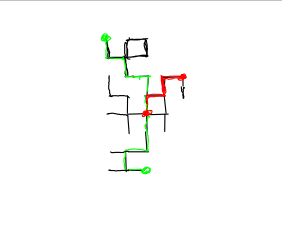
\includegraphics[width=.55\textwidth]{figures/definitions}
\caption{A typical percolation cluster is shown.  The chemical distance, or shortest path, between two arbitrary sites on the cluster is colored red; the diameter is colored green.}\label{fig:definitions}
\end{figure}

\begin{figure}[htp]
\centering
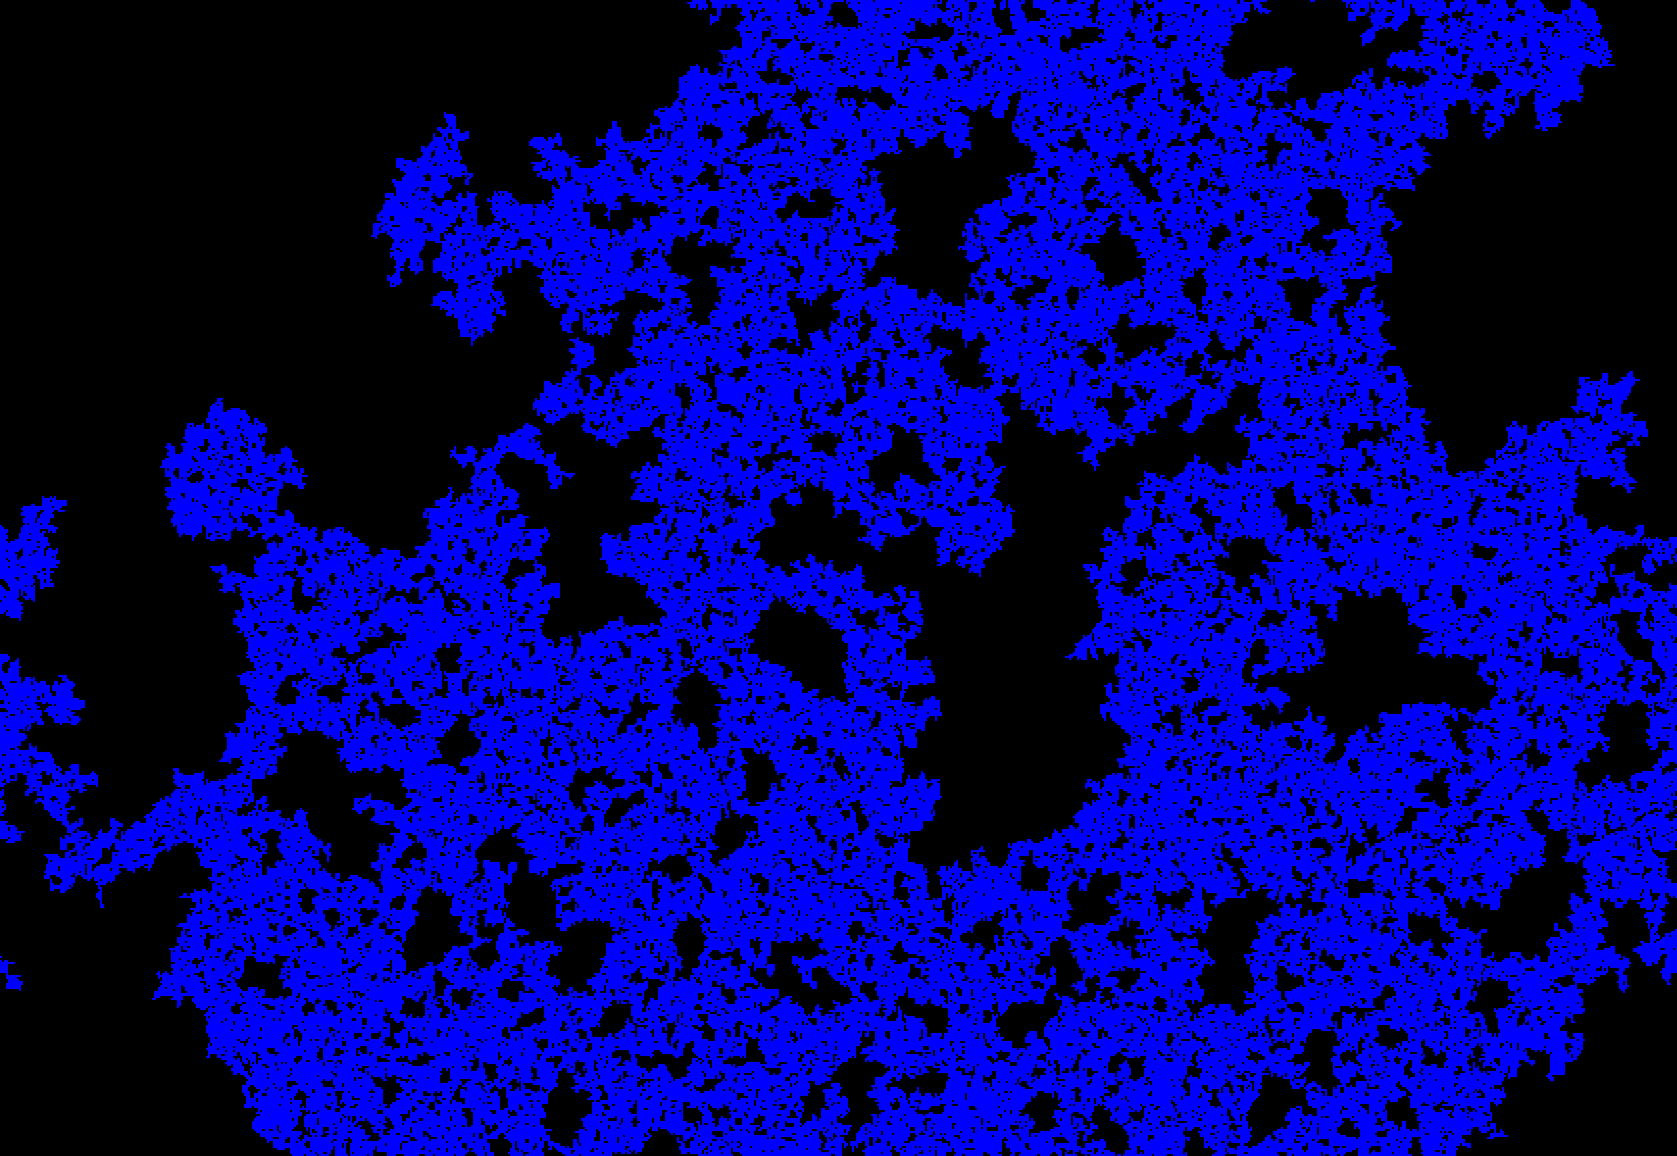
\includegraphics[width=.55\textwidth]{figures/pottscluster}
\caption{Example Potts Cluster, 2D, $q=1$ (Percolation).}
%\label{fig:pottscluster}
\end{figure}

\begin{figure}[htp]
\centering
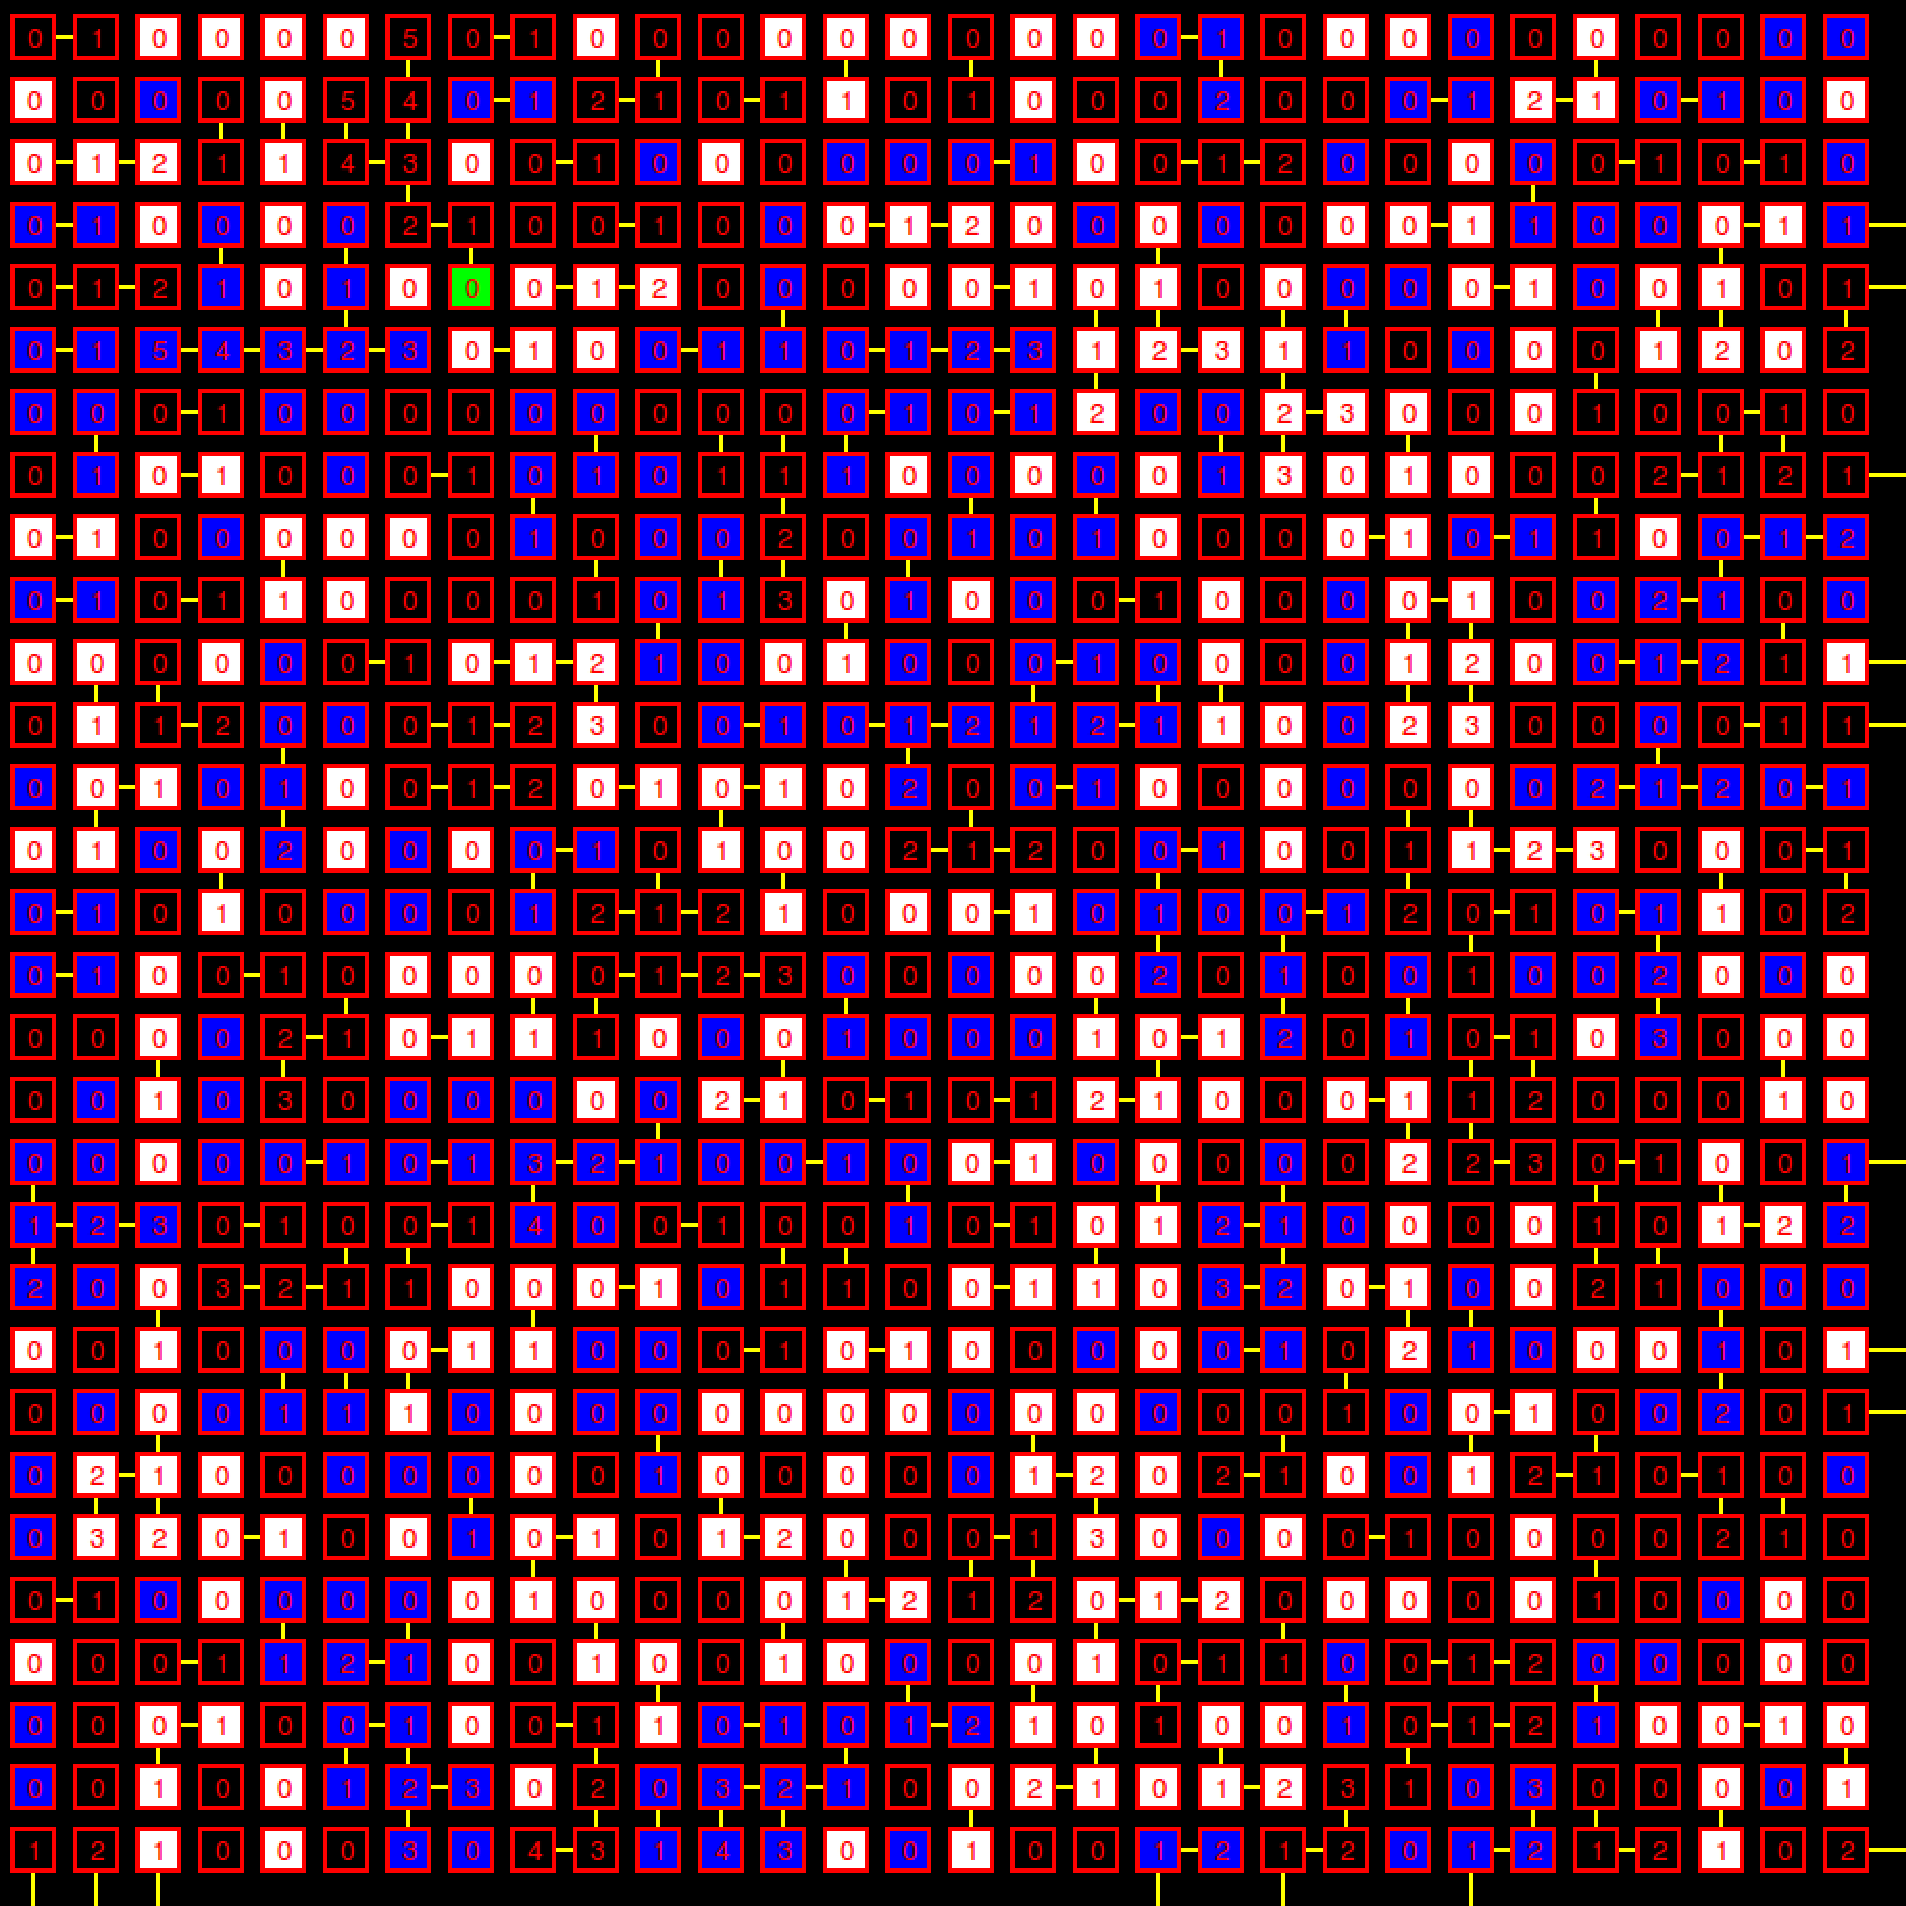
\includegraphics[width=.35\textwidth]{figures/q3potts}
\caption{Leath Growth Example, 2D, $q=1$.}
%\label{fig:shortest}
\end{figure}


\begin{figure}[htp]
\centering
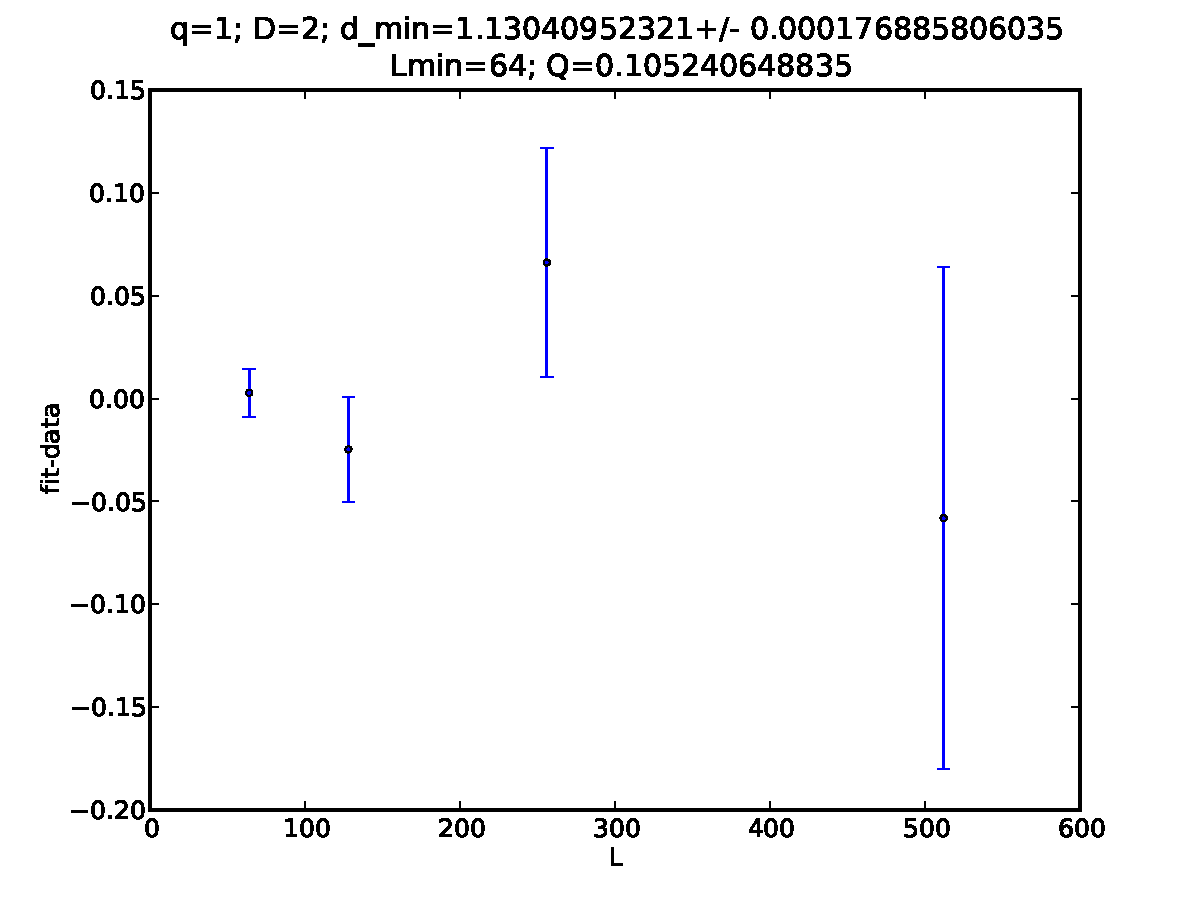
\includegraphics[width=.55\textwidth]{figures/q1D2Lmin64fitplot}
\caption{Residuals for $l$ and $w$, 2D Potts, $q=1$, fit of form $y=AL^B$.}
\end{figure}

\begin{figure}[htp]
\centering
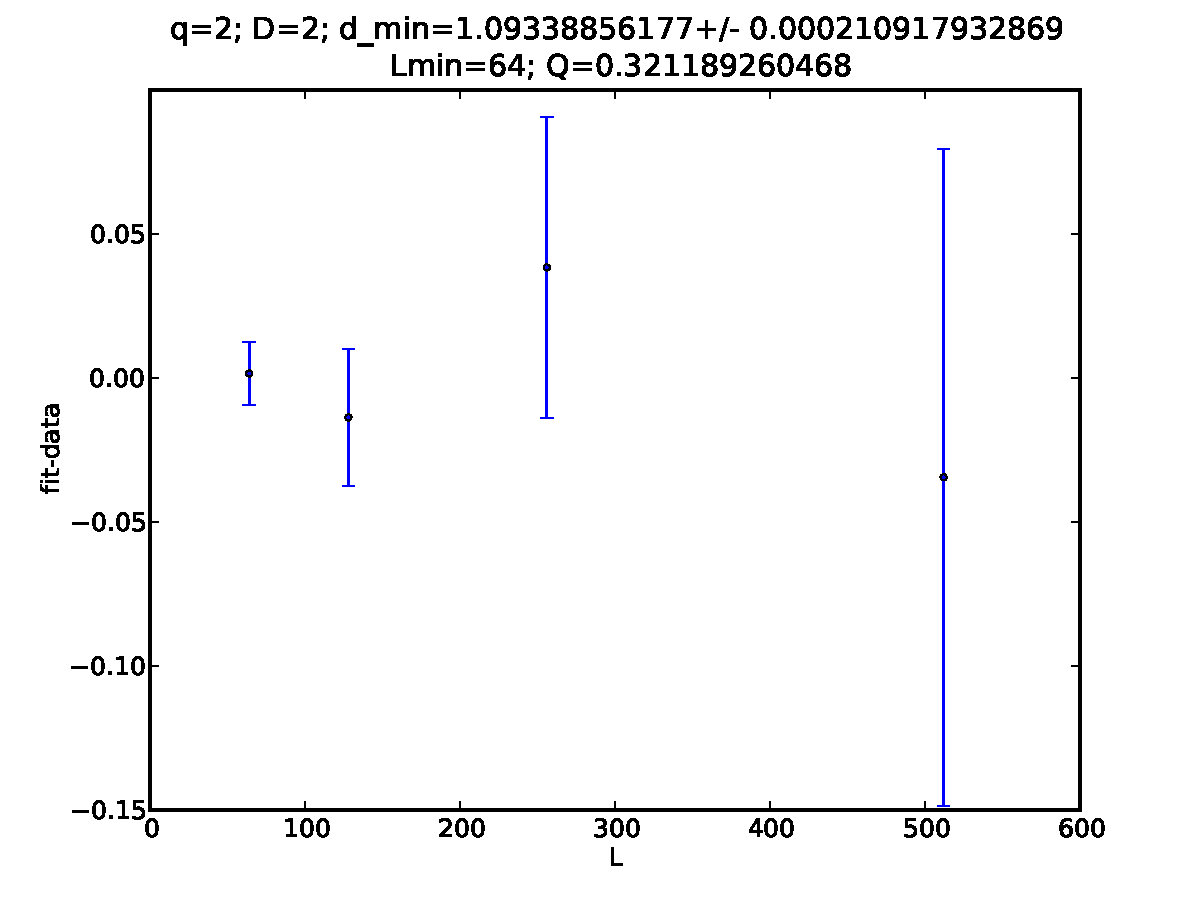
\includegraphics[width=.55\textwidth]{figures/q2D2Lmin64fitplot}
\caption{Residuals for $l$ and $w$, 2D Potts, $q=2$, fit of form $y=AL^B$.}
\end{figure}

\begin{figure}[htp]
\centering
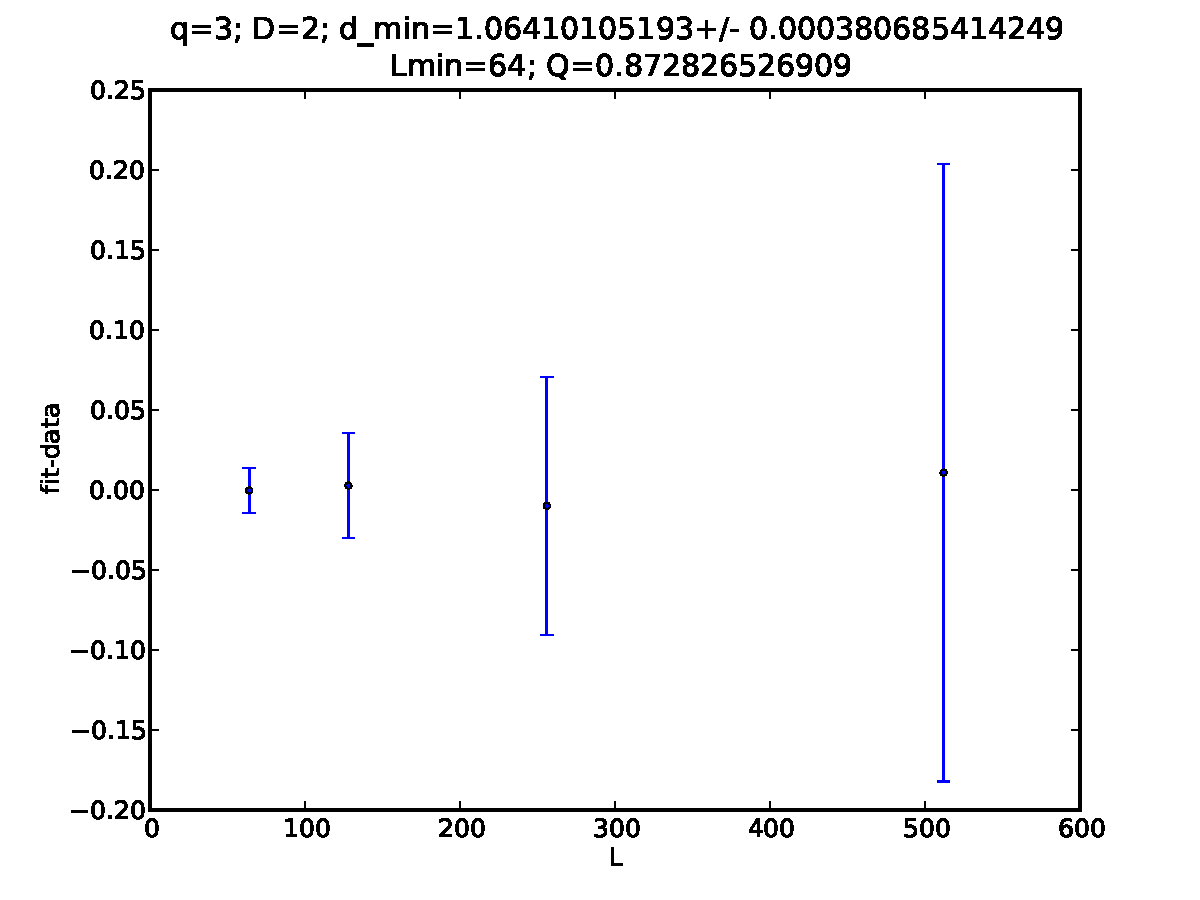
\includegraphics[width=.55\textwidth]{figures/q3D2Lmin64fitplot}
\caption{Residuals for $l$ and $w$, 2D Potts, $q=3$, fit of form $y=AL^B$.}
\end{figure}

\begin{figure}[htp]
\centering
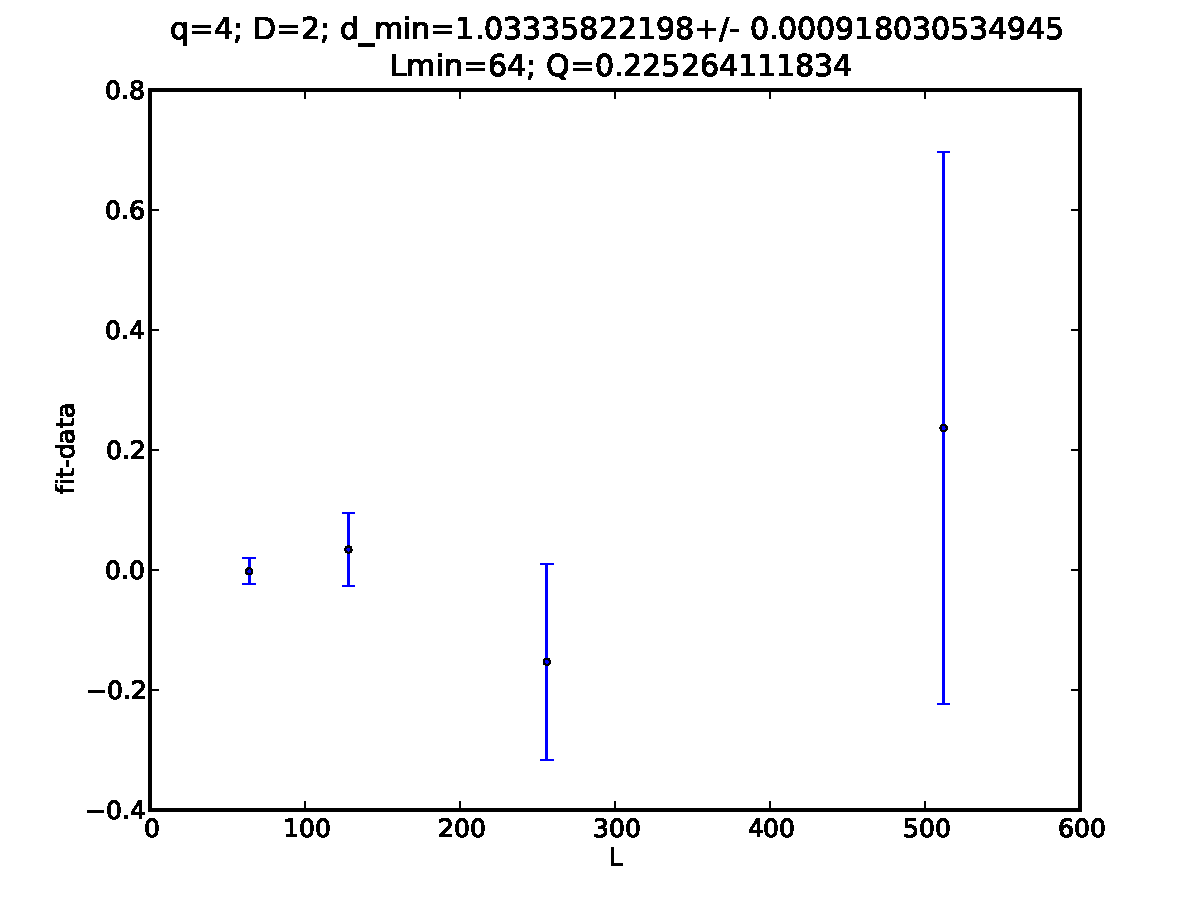
\includegraphics[width=.55\textwidth]{figures/q4D2Lmin64fitplot}
\caption{Residuals for $l$ and $w$, 2D Potts, $q=4$, fit of form $y=AL^B$.}
\end{figure}































% \subsection{Ways of measuring chem distance, diameter}

% \subsection{Mean field theory expectations}

% \subsection{Analysis techniques}


% \subsection{FIGURES:}


% \subsubsection{chemical distance and diameter, defined}

% \subsubsection{example cluster for q=1 or 2, chemical distance, diameter}

% \subsubsection{explanation of new diameter method}

% \subsubsection{Scaling of the chemical distance in 2D, Potts q=1,2,3,4}

% \subsubsection{Scaling of the chemical distance in q=2 in 4D, q=1 in 6D (necessary?)}

% \subsubsection{Scaling of the diameter in 2D, Potts q=1,2,3,4}

% \subsection{Results}

% \subsubsection{Scaling of the chemical distance in 2D, Potts q=1,2,3,4}


% \begin{description}

% \item[4 FIGURES:  residuals for scaling exponent for each value of q]\label{sec-2.4.1.1}


% \end{description}
% \begin{description}

% \item[comparison with Sokal's results]\label{sec-2.4.1.2}


% \end{description}
% \subsubsection{Scaling of the chemical distance in q=2 in 4D, q=1 in 6D (necessary?)}
% \label{sec-2.4.2}

% \begin{description}

% \item[Comparison with mean field theory]\label{sec-2.4.2.1}


% \end{description}
% \begin{description}

% \item[2 FIGURES:  residuals for q=2 \& q=1, here]\label{sec-2.4.2.2}


% \end{description}
% \subsubsection{Scaling of the diaemter in 2D, Potts q=1 -- high precision}
% \label{sec-2.4.3}

% \begin{description}

% \item[1 FIGURE: residuals]\label{sec-2.4.3.1}


% \end{description}
% \subsubsection{Scaling of the diameter in 2D, Potts q=1,2,3,4 -- comparison with chemical distance}
% \label{sec-2.4.4}




















% \section{Old Intro}
% \label{sec-3}

% \subsection{Background to the Potts Model}
% \label{sec-3.1}

% \subsection{Tests of the Potts Model}
% \label{sec-3.2}

% \subsection{This is all we need to know}
% \label{sec-3.3}

% \subsection{Not much more syntax highlighting}
% \label{sec-3.4}

% \subsubsection{Big test}
% \label{sec-3.4.1}

% \subsubsection{Other test}
% \label{sec-3.4.2}

% \subsubsection{Finish the damn outline}
% \label{sec-3.4.3}

% The Potts Model, initially introduced as a generalization of the 2-state Ising Model to $q$ possible spin states, can in fact be mapped onto the Random Cluster Model for all $q \ge 0$, with $q \to 1$ corresponding to the Percolation Model, and $q \to 2$ corresponding to the Ising Model.  The Potts Model has found application in an impressively diverse range of applications, including conformal field theory, percolation theory, knot theory, quantum groups, mathematical biology, and complex networks.    
% \%more specific \ldots{}    
% Although easy to formulate, the model exhibits rich phase behavior, and its study has yielded many significant insights into critical phenomena in statistical physics. 

% An important \textbf{geometric} property of Potts clusters that has proved very useful in describing transport and diffusion processes in random media is the ``chemical distance'', $l$ -- the length of the ``chemical'' or shortest path between two randomly chosen sites on a cluster.  The average chemical distance on critical Potts clusters has been shown to scale as $\bar{l} \propto r^{d_{min}}$ at criticality, where $r$ is the Euclidean distance between the endpoints of the chemical path $l$. Attempts to establish a relationship between $d_{min}$ and other known critical exponents have, as yet, proved inconclusive [refs]. 

% % For the $q \to 1$ (Percolation) case, much work has already been done to determine $d_{min}$ numerically \cite{Gr83, HrSt88} and an exact solution has been found using results from conformal field theory \cite{Zi99}.
 
% In this paper we generalize previous studies of $d_{min}$ for the 2D, $q=1$ Potts Model by reporting results for the $q = 2, 3$ and $4$ for both Potts Models in both 2D and 3D.  We also study the critical scaling of a related quantity: the diameter, $D$, defined as the longest of all the shortest paths between points on a cluster. (An illustration of both $D$ and $l$ on a Potts cluster is shown in Figure [A]).  We show that $D$ also exhibits scaling behavior at criticality: $\bar{D} \propto r^{w_{min}}$; and that, significantly, $d_{min} = D_{min}$ to within the error of our numerical results.  
 
% We also propose a possible relationship between both $D_{min}, d_{min}$ and the dynamical exponent, $z$.

% \begin{tabular}{lrr}
%  Name   &  Phone  &  Age  \\
% \hline
%  Peter  &   1234  &   17  \\
%  Anna   &   4321  &   25  \\
% \end{tabular}


% \section{Methods}
% \label{sec-4}

% \subsection{type 1}
% \label{sec-4.1}

% \subsection{type 2}
% \label{sec-4.2}

% \subsubsection{sub-sub}
% \label{sec-4.2.1}

% \begin{figure}[htp]
% \centering
% 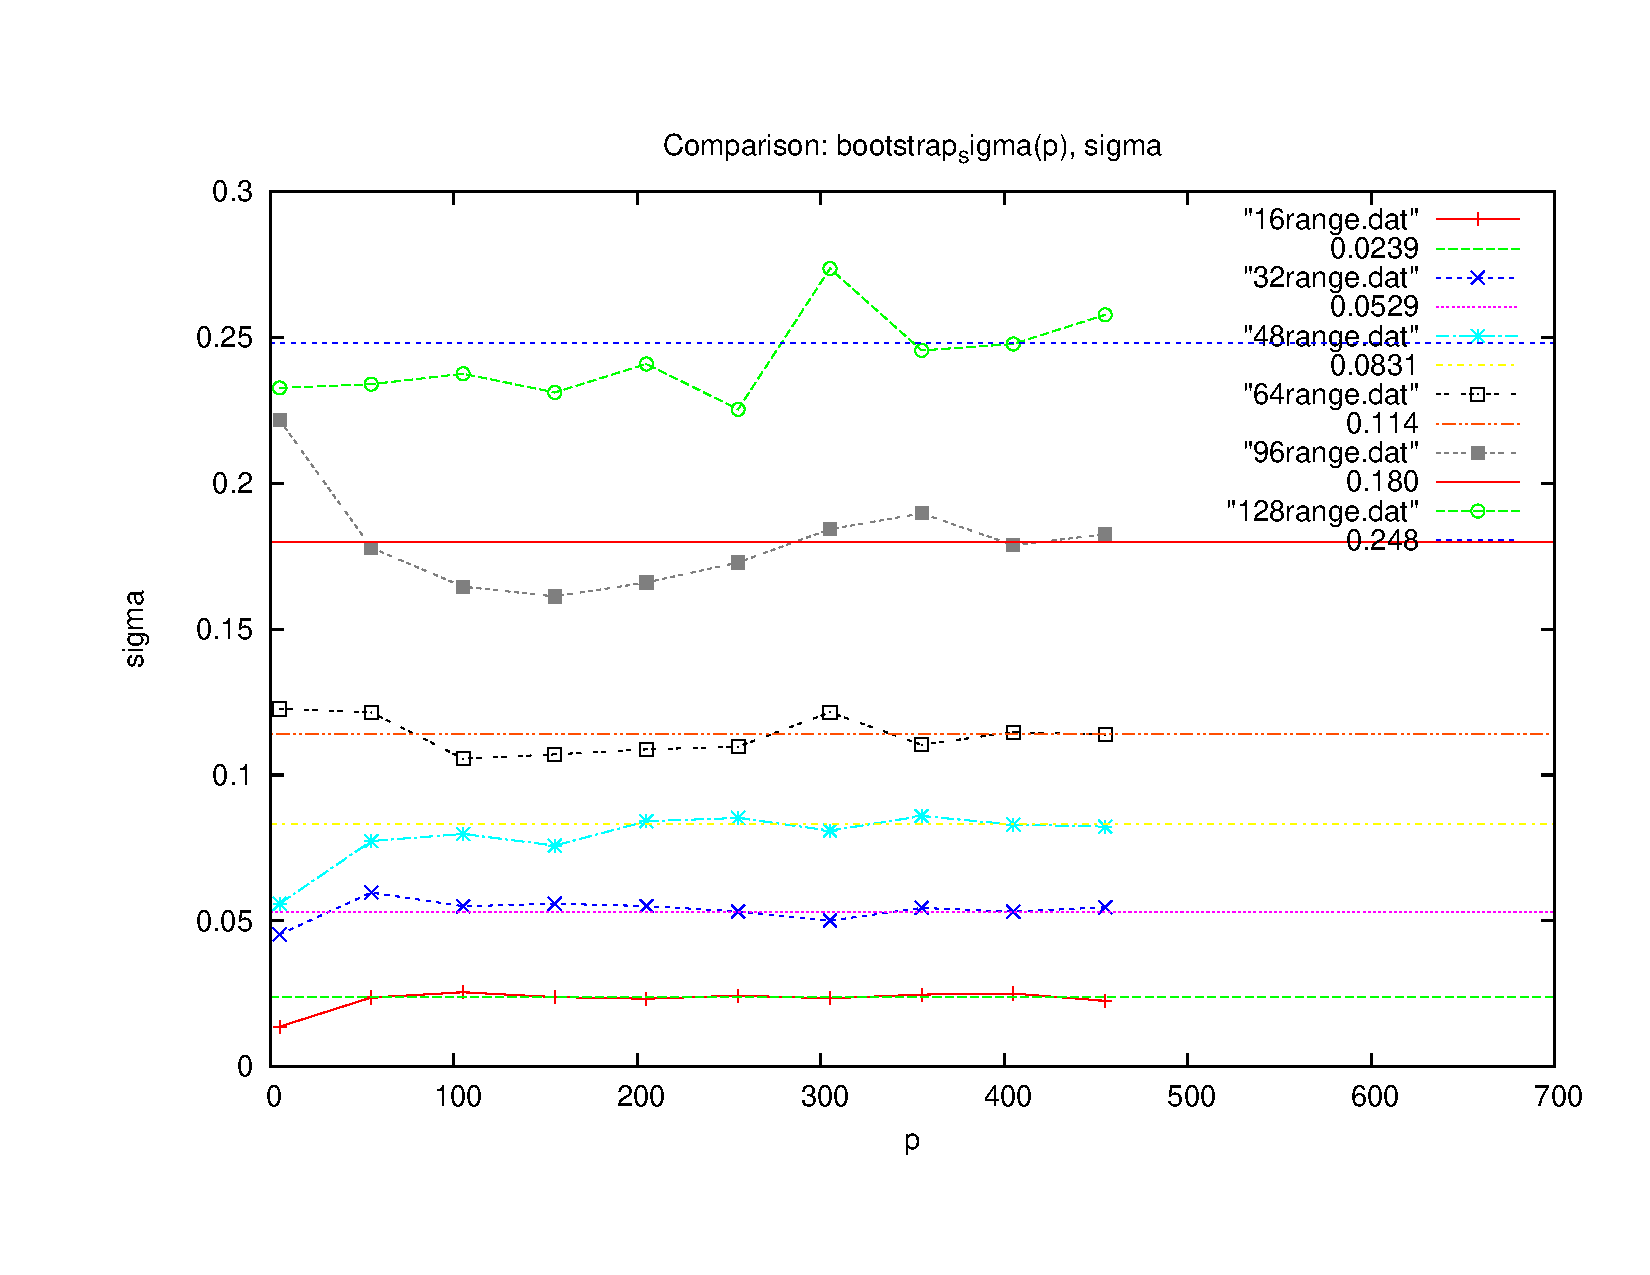
\includegraphics[width=.85\textwidth]{boot}
% \caption{$d_{min}$ for D=2, q=1.}\label{fig:1}
% \end{figure}


\section{Bibliography}
\label{sec-5}


\bibliographystyle{plain}
%\bibliography{/home/dwblair/Dropbox/dwbdocs/physics/writing/bibfiles/dwbreferences}
\bibliography{/home/dwblair/Dropbox/dwbdocs/physics/writing/bibfiles/combo}
\end{document}